\chapter{Additional Plots from NN Studies}

Various additional plots are shown in this appendix from the neural network creation and studies.  Figure \ref{fig:VarPlots4} and \ref{fig:VarPlots5} show additional shape comparisons in variables which are not included in the final neural network model as they do not significantly change the fit values.  In the cases of $p_T$ or $E$ variables with the higher separation value were used as there is a large correlation between the two values and the other is shown in this appendix.  $\Delta R_{jb}$ was not included as the other 3 $\Delta R$ values had higher separation values and they are all related to each other as they are the geometrically related. 

The neutrino reconstruction is done using a minimization of \[ \chi^2_{\nu} = \chi^2_{bW} + \chi^2_{W} \].  All three were investigated for their separation values and the $\chi^2_{W}$ value had the largest separation.

\begin{figure}[h!]
\centering
\subfloat[E (bjet)]{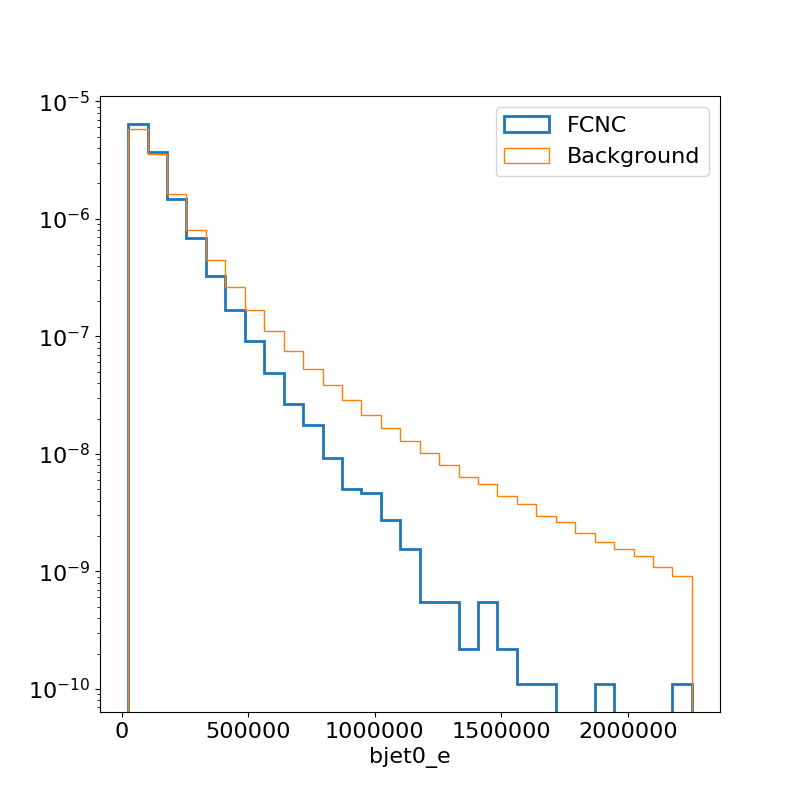
\includegraphics[width=.4\columnwidth]{../ThesisImages/SearchStrategy/varplots/bjet0_e.png}}\hfil
\subfloat[$\eta_b$]{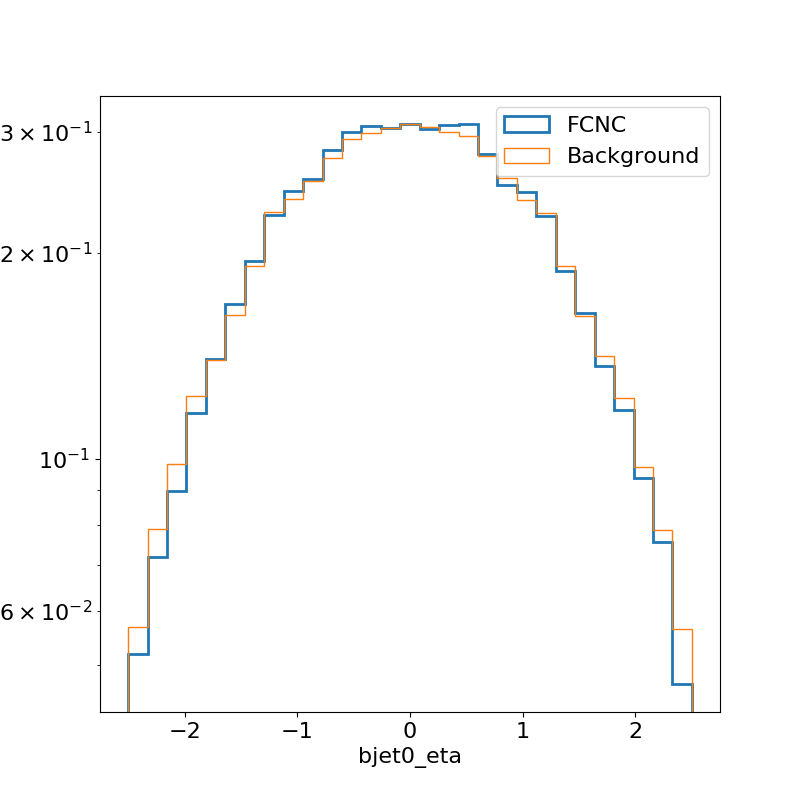
\includegraphics[width=.4\columnwidth]{../ThesisImages/SearchStrategy/varplots/bjet0_eta.png}}
\vspace{-4.5mm}
\subfloat[$\Delta R_{jb}$]{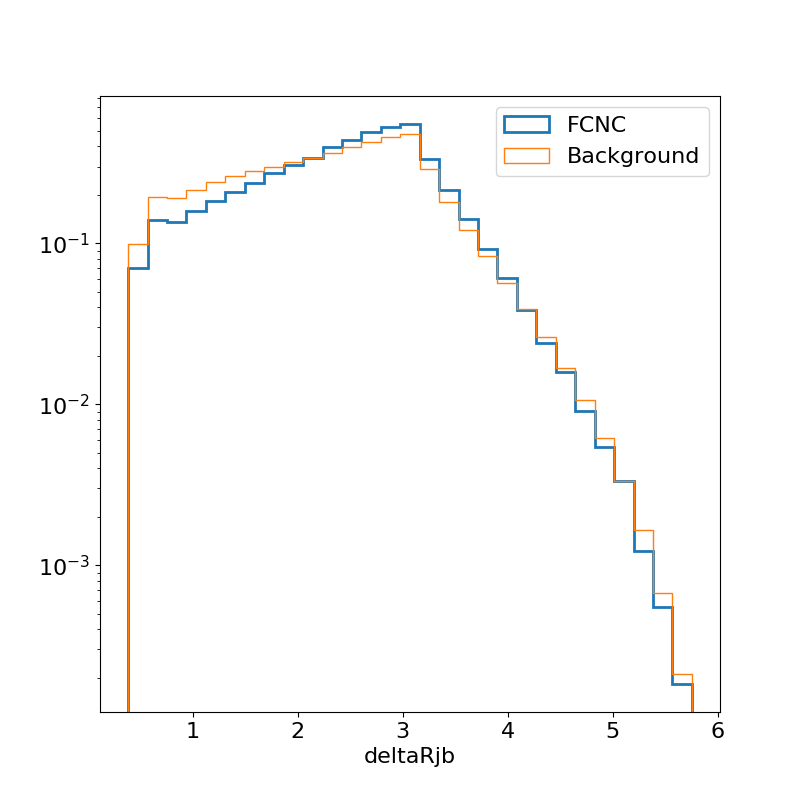
\includegraphics[width=.4\columnwidth]{../ThesisImages/SearchStrategy/varplots/deltaRjb.png}}\hfil
\subfloat[E (light jet)]{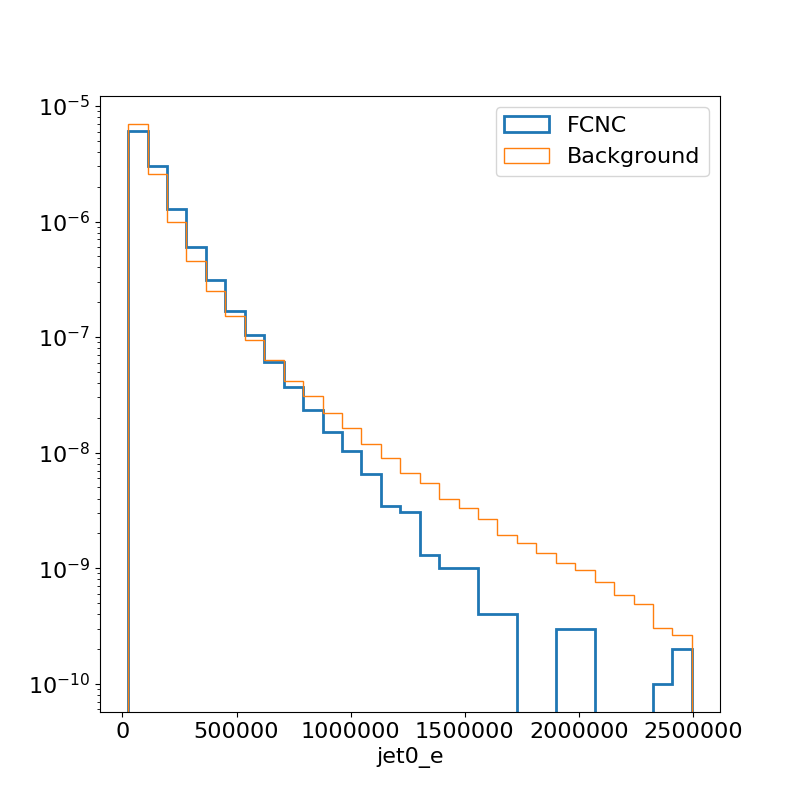
\includegraphics[width=.4\columnwidth]{../ThesisImages/SearchStrategy/varplots/jet0_e.png}}   
\vspace{-4.5mm}
\subfloat[light jet $\eta$]{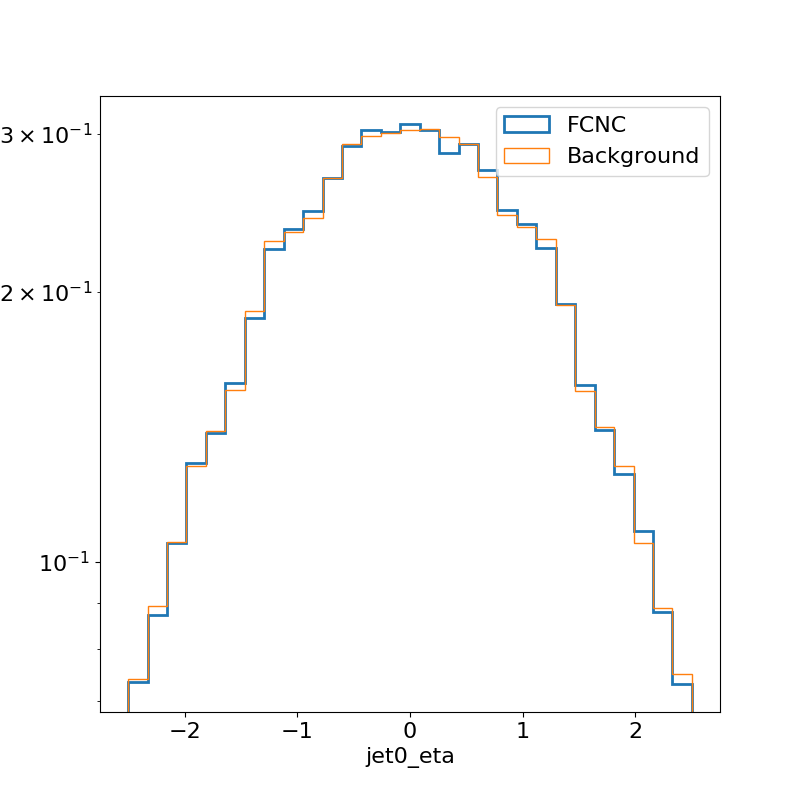
\includegraphics[width=.4\columnwidth]{../ThesisImages/SearchStrategy/varplots/jet0_eta.png}}\hfil
\subfloat[$\chi^2_\nu$]{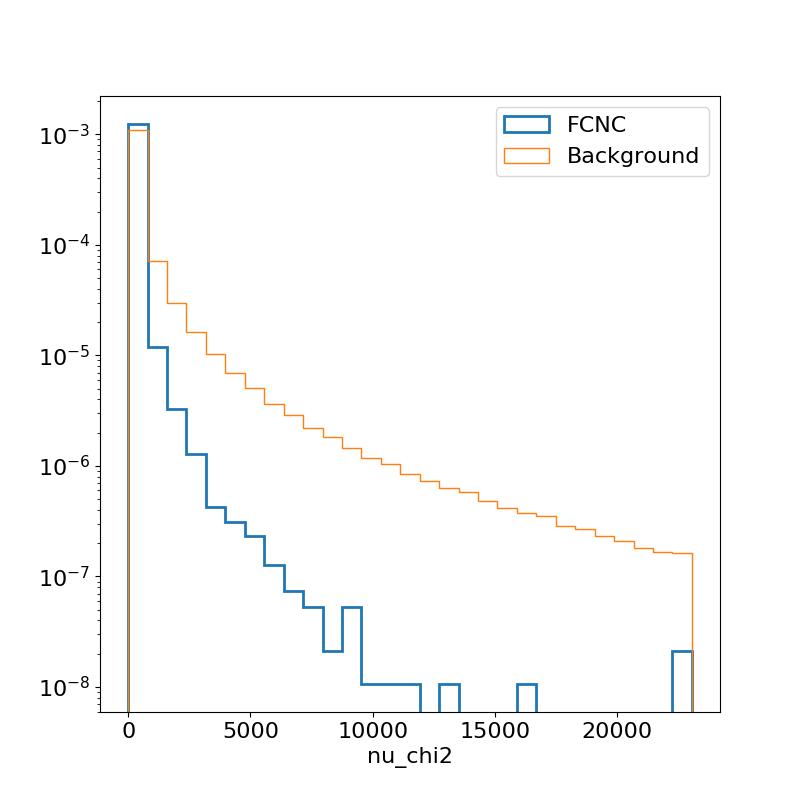
\includegraphics[width=.4\columnwidth]{../ThesisImages/SearchStrategy/varplots/nu_chi2.png}}
\caption{Normalized variables showing the shapes of neural network input variables: [E (bjet), $\eta_b$, $\Delta R_{jb}$ ,E (light jet), light jet $\eta$, and $\chi^2_\nu$ the total $\chi^2$ fit value  }
\label{fig:VarPlots4}
\end{figure}


\begin{figure}[h!]
\centering
\subfloat[lepton $p_T$]{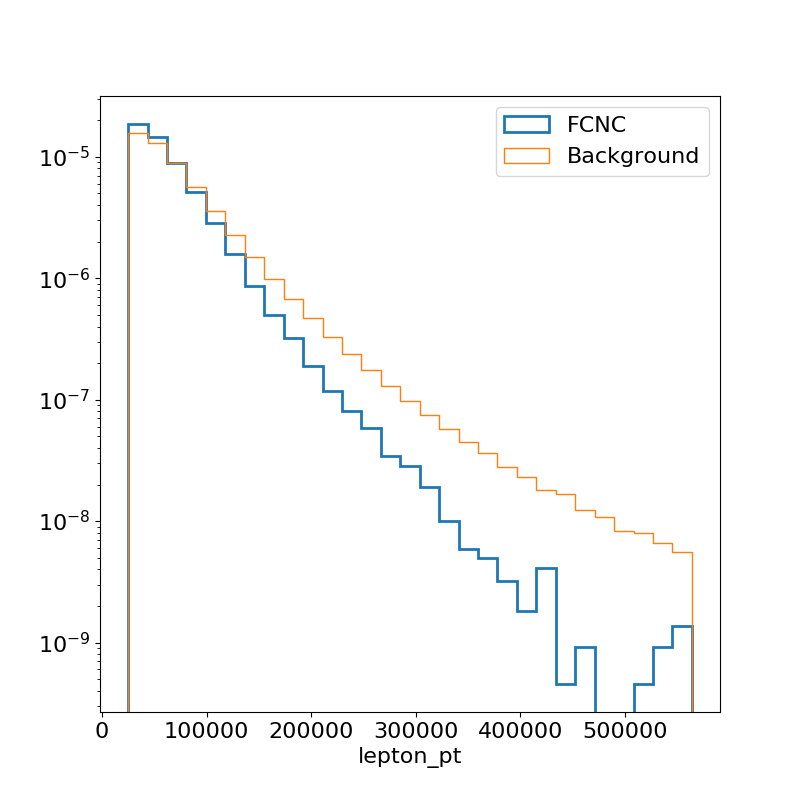
\includegraphics[width=.4\columnwidth]{../ThesisImages/SearchStrategy/varplots/lepton_pt}}\hfil
\subfloat[lepton $\eta$]{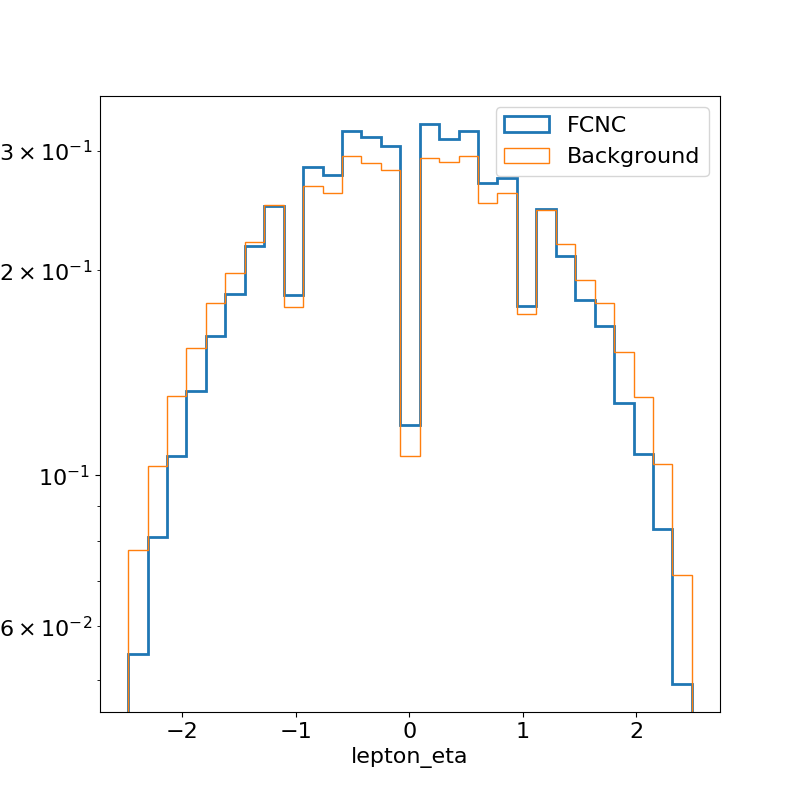
\includegraphics[width=.4\columnwidth]{../ThesisImages/SearchStrategy/varplots/lepton_eta.png}}
\vspace{-4.5mm}
\subfloat[lepton isolation]{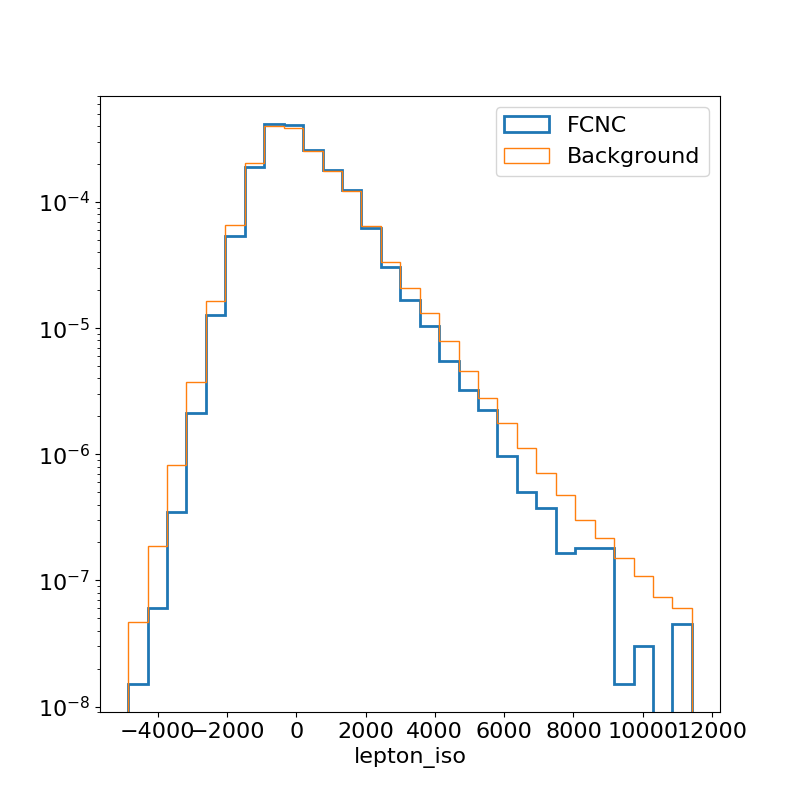
\includegraphics[width=.4\columnwidth]{../ThesisImages/SearchStrategy/varplots/lepton_iso.png}}\hfil
\subfloat[$\chi^2_{\text{bW}}$]{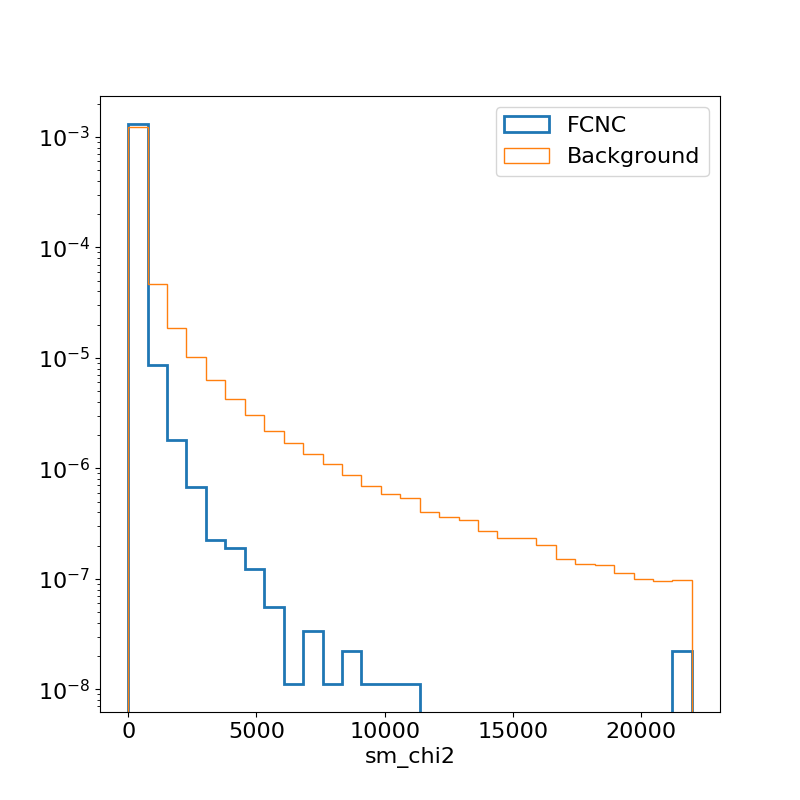
\includegraphics[width=.4\columnwidth]{../ThesisImages/SearchStrategy/varplots/sm_chi2.png}}   
\vspace{-4.5mm}
\subfloat[photon E]{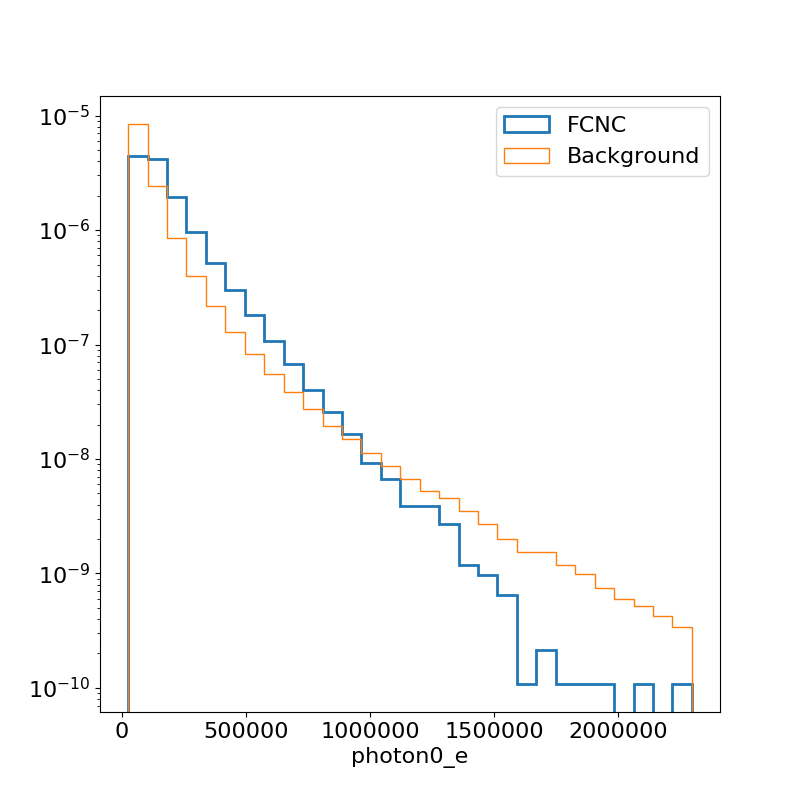
\includegraphics[width=.4\columnwidth]{../ThesisImages/SearchStrategy/varplots/photon0_e.png}}\hfil
\subfloat[photon $\eta$]{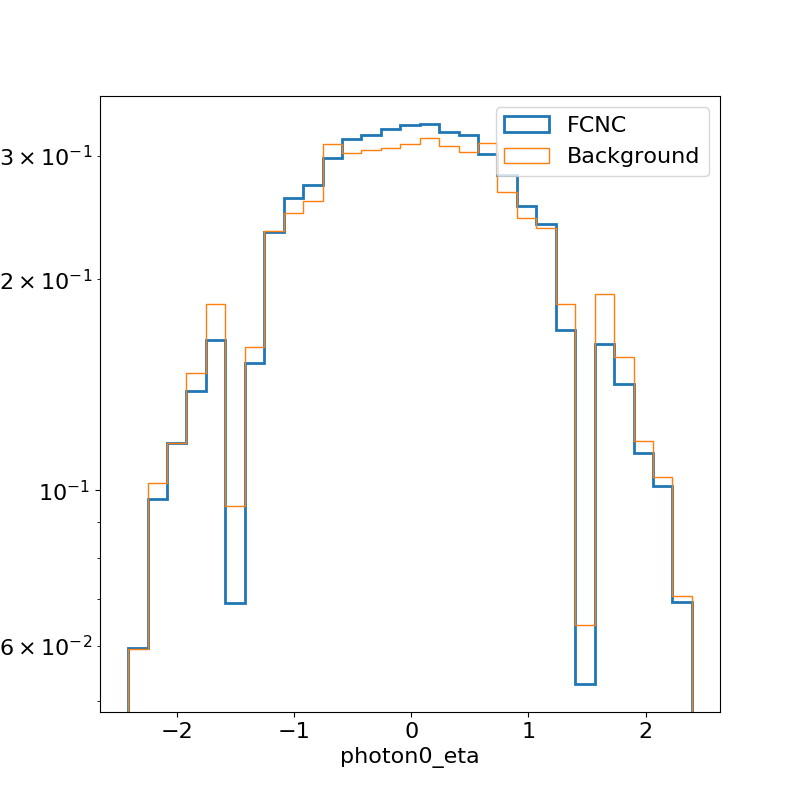
\includegraphics[width=.4\columnwidth]{../ThesisImages/SearchStrategy/varplots/photon0_eta.png}}
\caption{Normalized variables showing the shapes of neural network input variables: [lepton $p_T$, lepton $\eta$, lepton isolation , $chi^2_{\text{SM}}$ the bW$\chi^2$ value from neutrino reconstrucion ,photon E, and photon $\eta$.  }
\label{fig:VarPlots5}
\end{figure}